\section*{Introduction}

	Nous posons dans ce \coursun les concepts indispensables dont nous nous servirons dans les chapitres à venir, en tentant de répondre à deux questions :
	\begin{itemize}
		\item Que représente l’énergie ?
		\item Quelles formes d’énergie manipule-t-on dans une machine ?
	\end{itemize}\dontbreakpage \vspace{2em}

\section{Démarche}

	L’objectif de ce cours de thermodynamique est de décrire les caractéristiques physiques des principaux moteurs de l’industrie. Pour pouvoir décrire leurs performances et leurs limites, il nous faut commencer un étage plus bas, en nous posant d’abord des questions comme :
	
		\begin{itemize}
			\item Comment et pourquoi un moteur peut-il fonctionner ? Comment transformer de la chaleur en travail ?
			\item Comment peut-on refroidir un objet ? Comment peut-on inverser le sens spontané des transferts de chaleur ?
		\end{itemize}

	Or, pour pouvoir donner des réponses solides à ces questions, il faut bien maîtriser les notions de chaleur, de température, et de travail ; ainsi nous devons d’abord descendre encore quelques étages plus bas :
	
		\begin{itemize}
			\item Comment quantifie-t-on la chaleur et le travail dans une machine ?
			\item Comment un fluide peut-il recevoir ou fournir de l’énergie ?
			\item Que représentent l’énergie, la chaleur, et la température ?
		\end{itemize}

	Ces questions sont le cœur de ce que nous appelons \vocab{thermodynamique}, c’est-à-dire l’étude de la nature de la chaleur. Nous allons devoir commencer tout en bas, et nous remonterons progressivement jusqu’à pouvoir enfin expliquer pourquoi le rendement d’un moteur Diesel dépasse rarement \SI{40}{\percent}. En route !
	
\section{Notion d’énergie}

	\subsection{L’énergie}
	
		Nous nous attaquons d’emblée à l’une des notions les plus difficiles de toute la physique : l’\vocab{énergie}. 
		
		Nous observons que dans tous les phénomènes, lors de toutes les transformations que nous pouvons observer dans l’univers, il existe une grandeur qui ne varie pas. Cette grandeur quantifie une propriété abstraite (énergie vient du grec \textgreek{ἐνέργεια}, \textit{energeia}, soit «~activité~», «~opération~») qui peut prendre de multiples formes. %On peut penser la notion d’énergie comme étant la capacité à mettre un objet en mouvement.
		
		Nous avons appris à compter la quantité d’énergie présente dans n’importe quel volume arbitraire, et nous nous attachons à contrôler sa transformation d’une forme à une autre. Par exemple, l’énergie électrique stockée dans une batterie peut être transformée en travail dans un moteur électrique, ce qui peut servir à actionner un ascenseur, qui peut soulever une charge. Lors de toutes ces évolutions, la quantité totale d’énergie reste la même (\cref{fig_crashed_car}), un fait qui nous permet par exemple de quantifier la taille minimale de batterie nécessaire pour soulever une charge donnée.
		
		\begin{figure}
			\begin{center}
				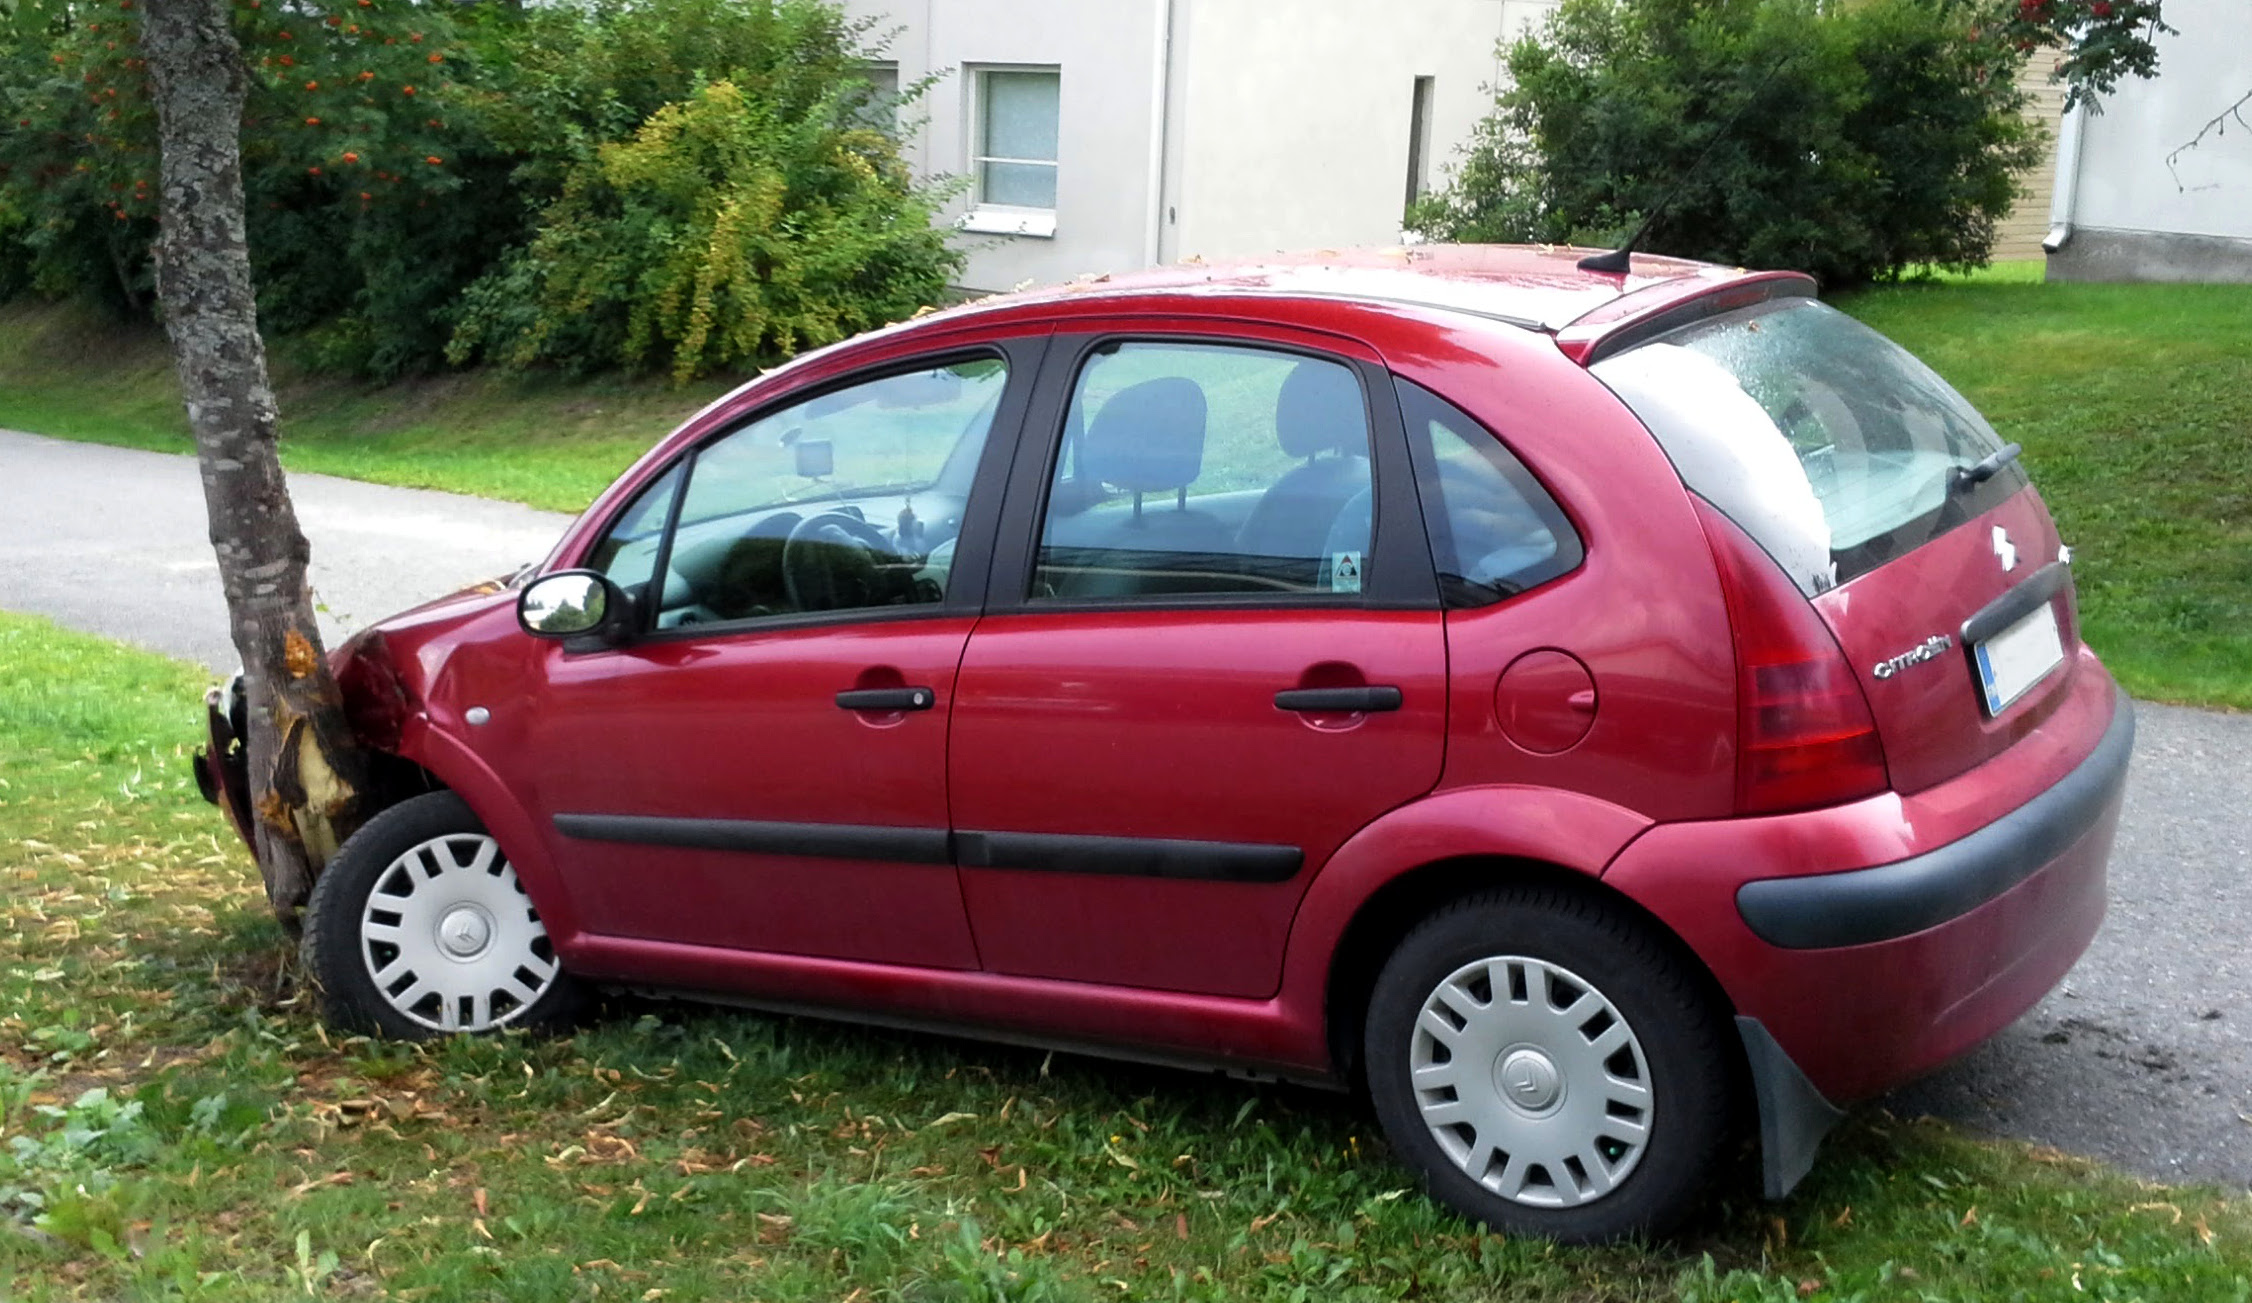
\includegraphics[width=0.5\textwidth]{images/crashed_citroen_c3.jpg}
			\end{center}
				\supercaption{L’énergie chimique stockée dans le carburant qui a été consommé est exactement égale à l’énergie rejetée par le pot d’échappement, plus l’énergie dissipée par frottement, plus l’énergie cinétique de la voiture en route. Toute cette énergie est transformée en chaleur, \emph{mais jamais détruite}, une fois la voiture arrêtée (quelqu’en soit le moyen !).}{Photo dérivée d’\wcfile{Crashed Citroën C3 (2).jpg}{une photo} \ccbysa par \wcun{Tommi_Nummelin}{Tommi Nummelin}}
			\label{fig_crashed_car}
		\end{figure}
		
		Ainsi, l’énergie est surtout un concept que nous utilisons pour lire les transformations que nous observons dans le monde : nous pourrions dire que c’est «~ce qui ne change pas lorsque les choses se transforment~». Pour l’ingénieur, elle représente surtout la capacité d’un corps à en mettre un autre en mouvement, de façon unifiée (par exemple avec un déplacement) ou désordonnée (par exemple avec une excitation chaotique). 

		Nous mesurons l’énergie en \si{joules} (\si{\joule}). 
	
	\subsection{Le premier principe}
		\label{ch_premier_principe}

		Le \vocab{premier principe de la thermodynamique} affirme simplement :

		\begin{principe}
				L’énergie est indestructible.
		\end{principe}

			\thermoquotebegin{O}
			Il est important de réaliser que dans la physique d’aujourd’hui, nous n’avons aucune connaissance de ce \emph{qu’est} l’énergie. Nous n’avons pas de représentation comme quoi l’énergie viendrait en petit paquets d’une certaine quantité. Cependant des formules permettent de calculer une quantité numérique, et lorsque nous les additionnons toutes, nous obtenons toujours le même nombre. C’est une chose abstraite en cela qu’elle ne nous donne pas le mécanisme ou les \emph{raisons} des différentes formules.
		\thermoquoteend{Richard Feynman, 1963}{\textit{The Feynman Lectures on \mbox{Physics}} \mbox{\cite{feynman1963, feynman1963fr}}}

		On peut aussi écrire que «~l’énergie de l’univers est constante~», ou «~l’énergie se conserve toujours~» : elle ne peut être ni créée ni détruite. Autrement dit, lorsqu’un objet reçoit un \si{joule} d’énergie, il peut soit l’emmagasiner, soit le re-fournir à l’extérieur ; mais en aucun cas il ne peut le détruire.

		Il n’y a que deux principes importants en thermodynamique ; le second (auquel nous consacrons les chapitres \sept et \huit) porte lui aussi sur la nature de l’énergie. Leurs implications sont énormes et ils sont le fruit d’un travail intellectuel profond et laborieux, long de plusieurs siècles. Il n’existe pas de preuve ou de démonstration de leur véracité, mais toutes nos observations et expériences les corroborent, de sorte qu’ils sont aujourd’hui universellement acceptés.
		
		Nous exprimerons quantitativement le premier principe de deux façons différentes, l’une pour un système fermé (au \coursdeuxshort, \cref{eq_premier_principe_sf_min}) et l’autre pour un système ouvert (au \courstroisshort, \cref{eq_petite_sfee_deltas_h}).
	
	
	\subsection{Formes d’énergie}
	
		Les différentes formes d’énergie que nous identifions usuellement ont été mises au jour une à une au cours de l’histoire de la physique.
		
		L’\vocab{énergie cinétique} est possédée par un corps du fait de sa vitesse (\textit{cf.} \cref{ch_energie_mecanique} plus bas). C’est la forme d’énergie la plus facile à identifier. Elle a longtemps été nommée \textit{vis viva} («~force vive~»).
		
		L’\vocab{énergie potentielle} est stockée avec l’interaction entre deux objets liés par une force dite conservative\footnote{Une force est dite \vocab{conservative} lorsqu’elle reste la même dans un sens comme dans un autre. Par exemple, le poids est conservatif (il est le même que l’on monte ou que l’on descende) mais le frottement ne l’est pas (il s’oppose toujours au mouvement).}. À l’échelle macroscopique, la forme la plus palpable est l’énergie potentielle d’altitude, issue du travail fourni à une masse contre son poids (c’est ce travail qui rend plus fatigante la montée d’escaliers que leur descente, par exemple). En écrasant un ressort, on y stocke de l’énergie potentielle de compression, que l’on récupère en le détendant.

		L’\vocab{énergie chimique} est une combinaison d’énergie potentielle et d’énergie cinétique \emph{entre atomes}. Le métabolisme humain est fondé sur des transferts énergétiques chimiques, tout comme la combustion des hydrocarbures avec l’oxygène atmosphérique, qui alimente presque tous nos véhicules.
		
		Au cours du \textsc{xx}\ieme siècle, on a découvert au niveau sub-atomique que la masse était aussi une forme d’énergie (ainsi le fameux $E = m c^2$ lie masse et énergie). L’énergie rayonnante (électromagnétique) est également identifiable au niveau sub-atomique. Ces formes d’énergie ne nous concernent pas dans cet ouvrage.

		En thermodynamique, nous allons nous concentrer sur trois formes d’énergie, identifiables à l’échelle macroscopique :
		
		\begin{description}
			\item [L’\vocab{énergie interne}] notée $U$, un concept que nous utilisons pour regrouper toute l’énergie cinétique et potentielle des molécules d’un corps. Elle représente la quantité totale d’énergie mécanique stockée à l’intérieur d’un objet ;
			\item [La \vocab{chaleur}] notée $Q$, qui est un transfert représentant la transmission d’énergie cinétique de manière chaotique d’un corps vers un autre ;
			\item [Le \vocab{travail}] noté $W$, qui est un transfert représentant la transmission d’énergie de manière cohérente d’un corps vers un autre.
		\end{description}

		D’une façon générale, l’ingénieur/e thermodynamicien/ne souhaite capter de la chaleur à des corps qu’il/elle veut refroidir, ou bien fournir du travail à des corps qu’il/elle veut déplacer. Nous allons donc étudier en détail ces transferts.
	
	\subsection{La puissance}

		La \vocab{puissance} représente un débit d’énergie dans le temps. Son unité \textsc{si} est le \si{joule} \si{par} \si{seconde}, c’est-à-dire le \si{watt} (\si{\watt}) :
		\begin{equation}
		\SI{1}{\watt} \equiv \SI{1}{\joule\per\second}
		\label{def_puissance}
		\end{equation}

		\begin{figure}
			\begin{center}
			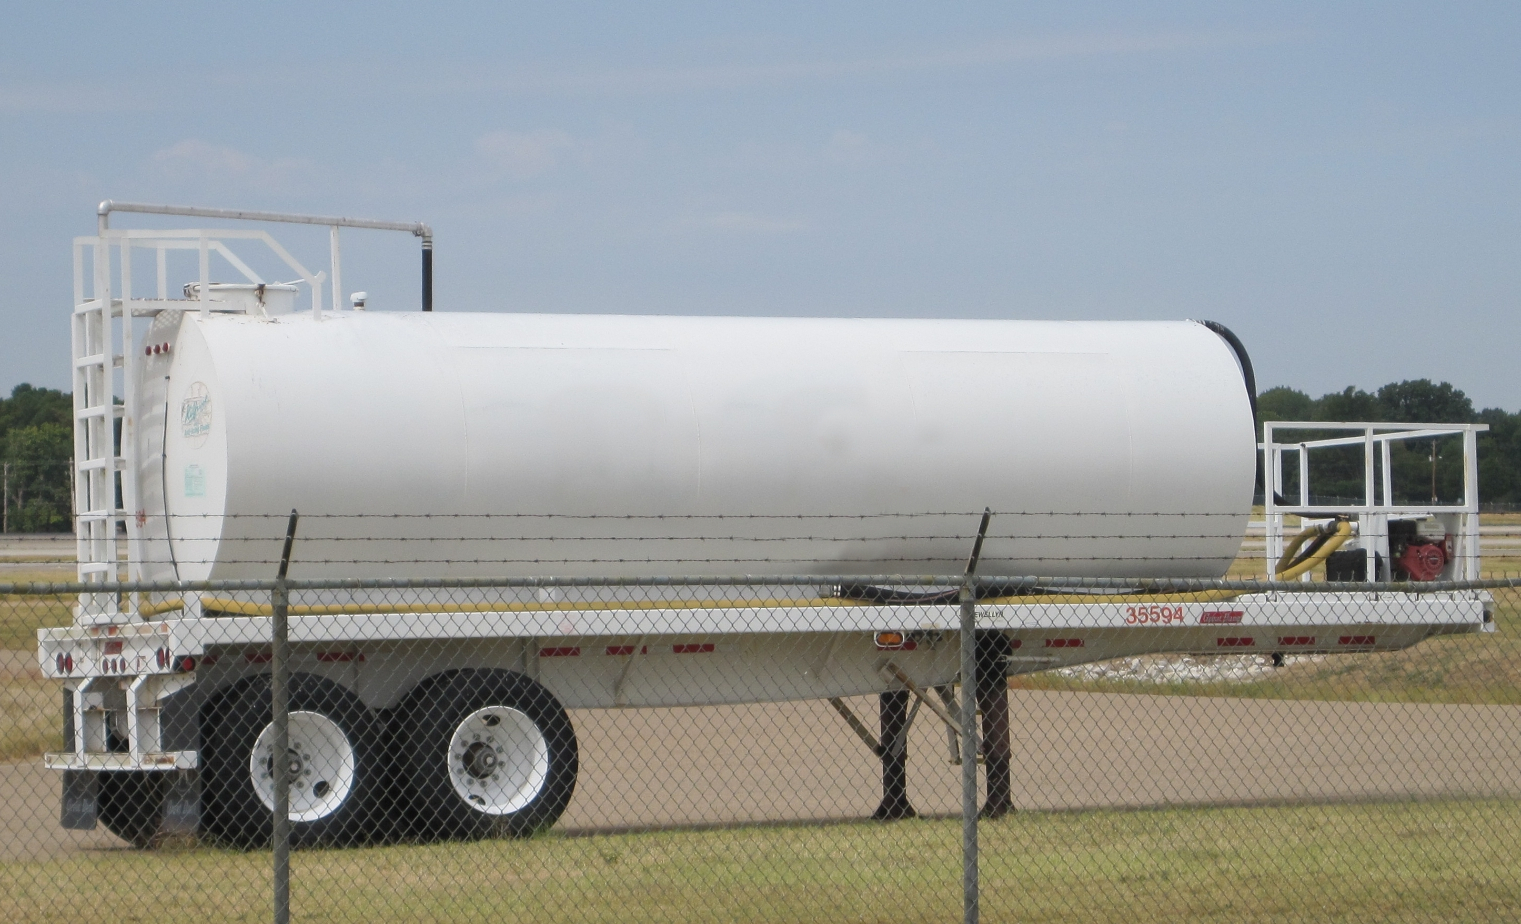
\includegraphics[height=0.31\textwidth]{images/fueltank.jpg}
			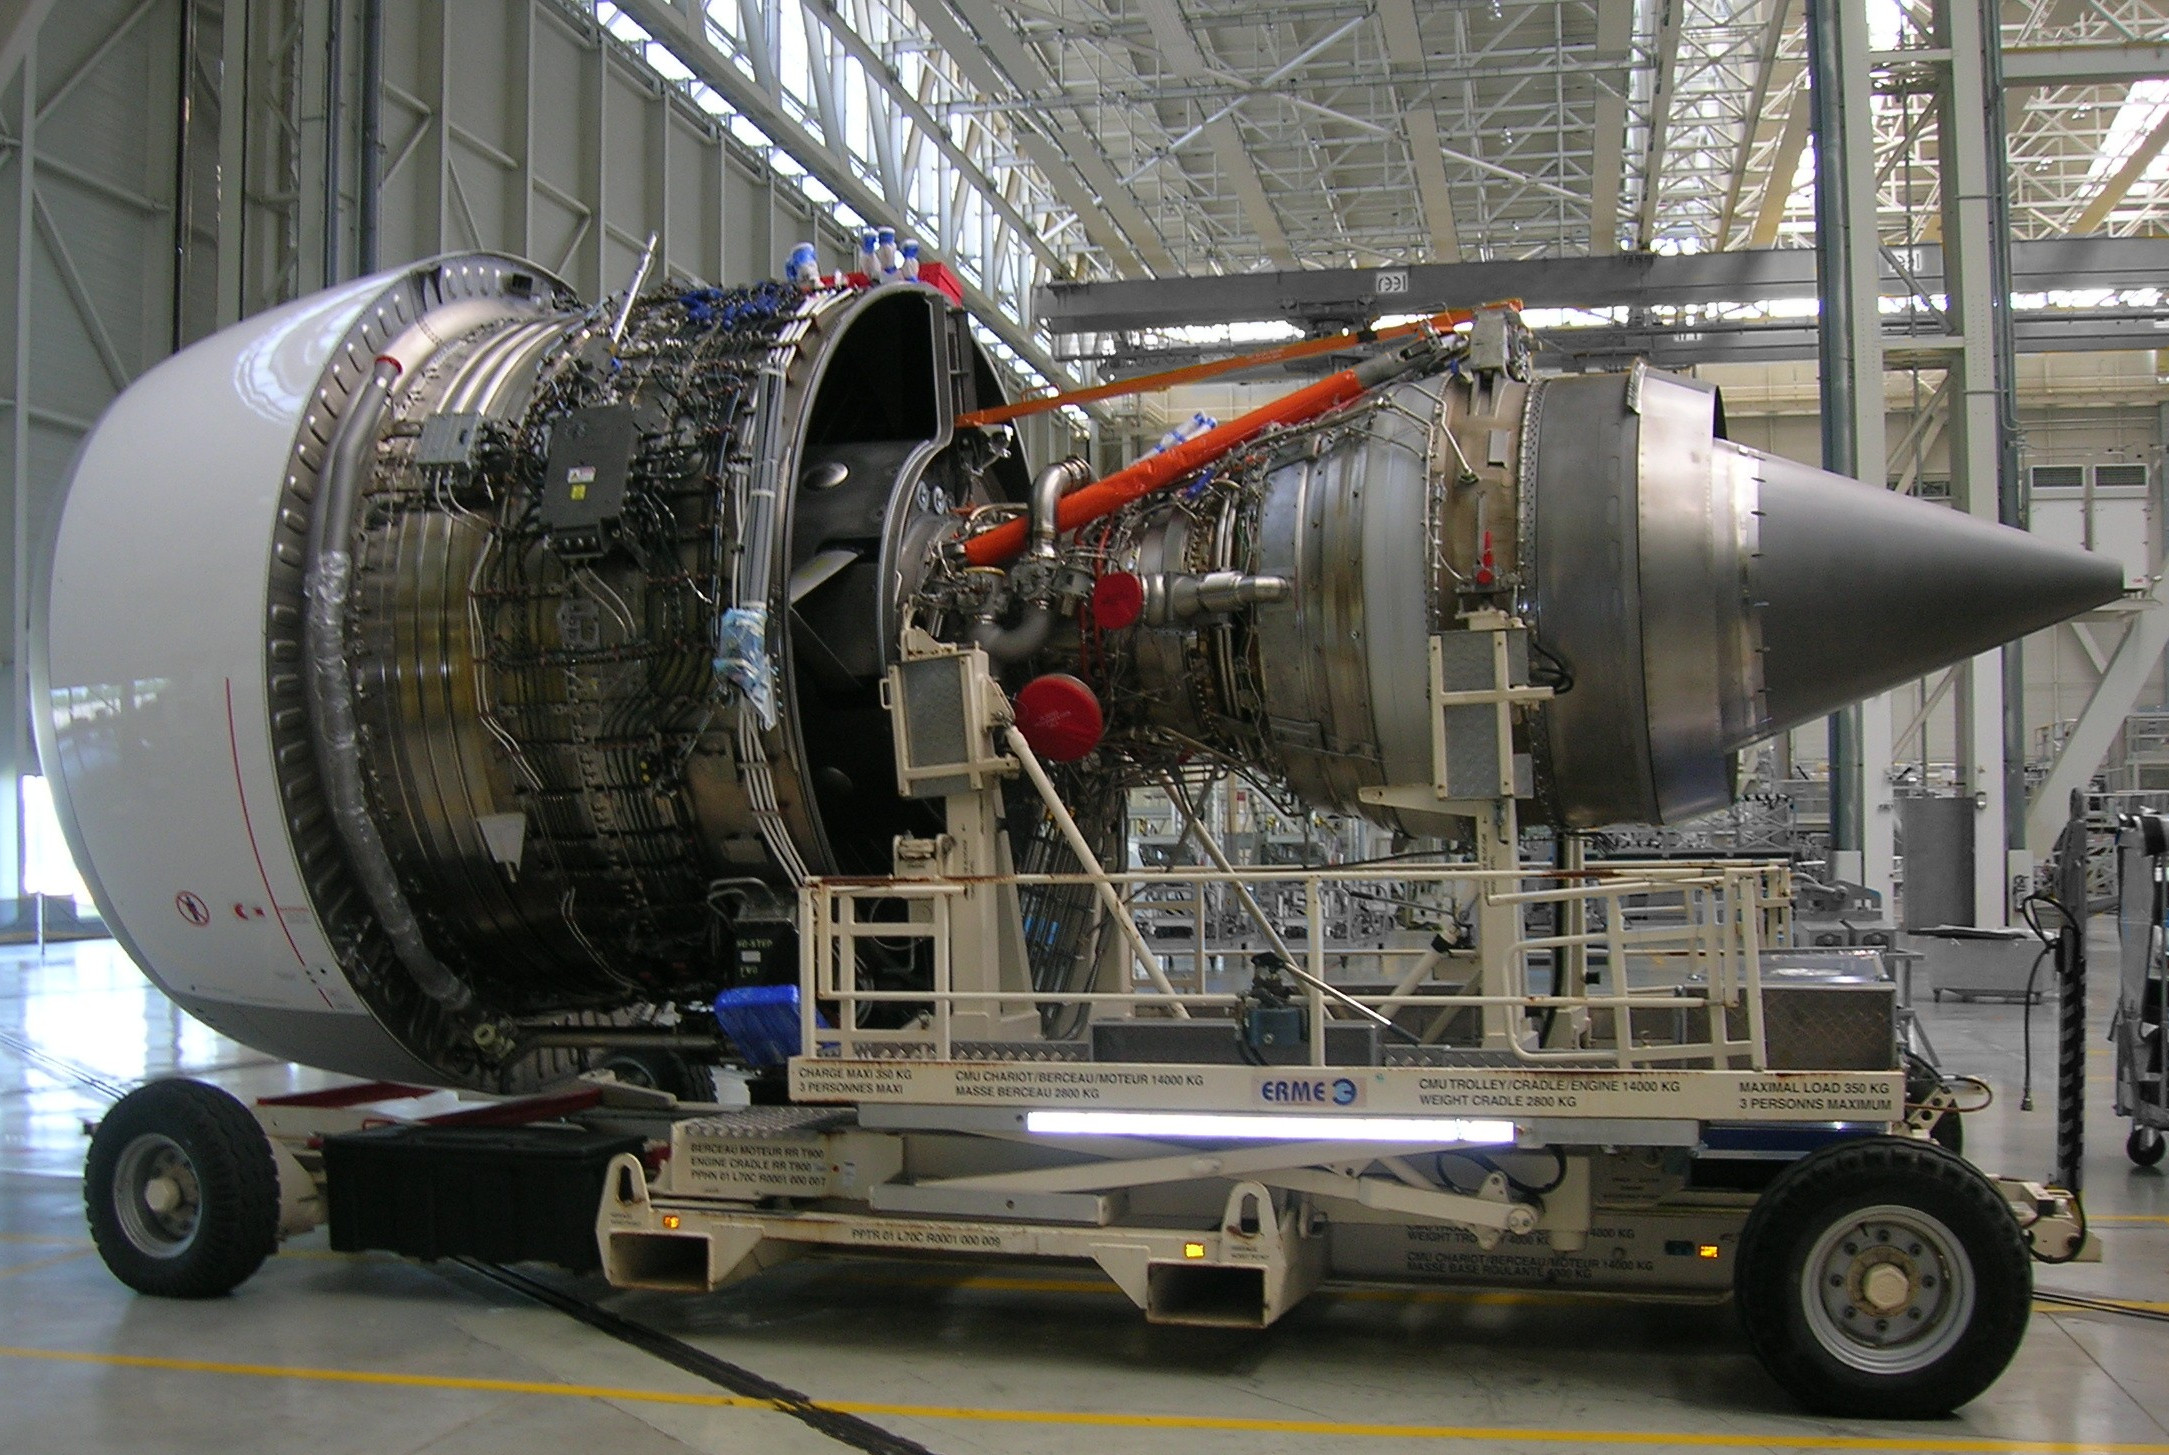
\includegraphics[height=0.31\textwidth]{images/trent900.jpg}
			\end{center}
			\supercaption{Une remorque, de puissance nulle ($\dot Q = \SI{0}{\watt}$) mais capable de restituer beaucoup d’énergie. La combustion de \SI{20}{\tonne} de kérosène dégage environ $Q = \SI{900}{\giga\joule}$ sous forme de chaleur ; \\
				Un turboréacteur à soufflante \textit{Trent 900}, de très grande puissance (capable de fournir $\dot W = \SI{20}{\mega\watt}$ à un avion de ligne) mais dépourvu d’énergie (\SI{0}{\joule}).}{Photo turboréacteur dérivée d’\wcfile{Airbus_Lagardère_-_Trent_900_engine_MSN100_(2).JPG}{une photo} \cczero par \wcu{Dr Brains}\\ Photo remorque dérivée d’\wcfile{FedEx_Express_fuel_tank_trailer_at_Memphis_International_Arirport.jpg}{une photo} \ccby Thomas R Machnitzki}
			\label{fig_energie_puissance}
		\end{figure}
		
		D’autres unités sont souvent utilisées, comme le cheval-vapeur%
			\footnote{Un cheval-vapeur correspond approximativement à la puissance que peut fournir sous forme de travail un cheval puissant en plein effort. Nous devons la création de cette unité à… James Watt (\S\ref{ch_cheval_vapeur}). Attention, il existe plusieurs définitions incompatibles de l’unité \textit{cheval}. L’\cref{eq_equivalence_cheval} correspond à la norme \textsc{din} 66036 utilisée dans l’industrie automobile.} : 
		\begin{equation}
			\SI{1}{ch_M} = \SI{735,5}{\watt}
			\label{eq_equivalence_cheval}
		\end{equation}

		Nous dénoterons les puissances avec un point au-dessus du symbole de l’énergie ; ainsi on note $\dot{E}$ \ une puissance (par exemple mécanique) apportant une quantité d’énergie $E$ chaque seconde.

		Dans le langage courant, le terme \textit{puissance} est utilisé pour quantifier \textit{la puissance maximale utile} d’un système. Par exemple, une automobile dont on dit qu’elle est «~de puissance 100~chevaux~» a un moteur capable de lui fournir, pendant quelques instants, une puissance de $\dot W_{\text{méca.}} = \SI{100}{ch}$ -- mais pour cela, le moteur reçoit environ $\dot Q_{\text{combustion}} = \SI{300}{ch}$ sous forme de chaleur. En outre, sur route, la puissance mécanique moyenne fournie par le moteur ne dépasse probablement pas \SI{20}{ch}.

	\subsection{L’énergie et la puissance massiques}
	\label{ch_valeurs_spécifiques}

		Dans de nombreuses applications en thermodynamique, il est intéressant de quantifier les transferts énergétiques indépendamment de la quantité de masse à l’intérieur de la machine. 

		Par exemple, si l’on souhaite comparer le \emph{fonctionnement} du moteur d’une moto et de celui d’un camion, il sera judicieux de diviser chacun des transferts énergétiques (compression, combustion, détente, etc) par la quantité d’air dans les cylindres, pour s’affranchir des effets d’échelle.

		À cet effet, nous utilisons des grandeurs dites \vocab{spécifiques} (dites parfois \vocab{massiques}) ; et nous les noterons en minuscules.

		\begin{description}
		
			\item[L’énergie spécifique] (parfois appelée énergie massique), se mesure en \si{joules} \si{par} \si{kilogramme}~(\si{\joule\per\kilogram}) :

				\begin{equation}
					e \equiv \frac{E}{m}
				\label{def_énergie_spécifique}
				\end{equation}

				\begin{equationterms}
					\item où \tab $e$ \tab est l’énergie spécifique (\si{\joule\per\kilogram}),
					\item \tab $E$ \tab l’énergie (\si{\joule}),
					\item et \tab $m$ \tab la masse du système que l’on étudie (\si{\kilogram}).
				\end{equationterms}
		
				\begin{anexample}
					Un injecteur d’essence dans un moteur de voiture doit fournir une quantité de chaleur spécifique $q_{\text{comb.}} = \SI{300}{\kilo\joule\per\kilogram}$ quelle que soit la quantité d’air dans le cylindre. Quelle sera l’énergie fournie lorsque $m_\text{air} = \SI{0,5}{\kilogram}$ et lorsque $m_\text{air} = \SI{1}{\kilogram}$ ?
		
					\begin{answer}Il faudra $Q_{\text{comb.}1} = m_1 q_{\text{comb.}} = \num{0,5} \times \num{300e3} = \num{150e3} = \SI{150}{\kilo\joule}$ dans le premier cas, et $Q_{\text{comb.}2} = m_2 q_{\text{comb.}} = \SI{300}{\kilo\joule}$ dans le second.\end{answer}
					\end{anexample}

		\item[La puissance spécifique] (parfois également appelée puissance massique), a les mê\-mes unités : on divise des \si{watts} (\si{joules} \si{par} \si{seconde}) par un débit de masse (\si{kilos} \si{par} \si{seconde}).
			\begin{equation}
				e \equiv \frac{\dot{E}}{\dot{m}}
				\label{def_puissance_spécifique}
			\end{equation}

			\begin{equationterms}
				\item où \tab $e$ \tab est la puissance spécifique (\si{\joule\per\kilogram}),
				\item \tab $\dot{E}$ \tab la puissance (\si{\watt}),
				\item et \tab $\dot{m}$ \tab le débit de masse traversant le système (\si{\kilogram\per\second}).
			\end{equationterms}

			\begin{anexample}
				Une chambre de combustion dans un turboréacteur doit fournir une quantité de chaleur spécifique $q_{\text{comb.}} = \SI{300}{\kilo\joule\per\kilogram}$ quel que soit le débit d’air traversant le moteur. Quelle sera la puissance fournie lorsque $\dot{m}_\text{air} = \SI{0,5}{\kilogram\per\second}$ et lorsque $\dot{m}_\text{air} = \SI{1}{\kilogram\per\second}$ ?
		
				\begin{answer}Il faudra une puissance $\dot{Q}_{\text{comb.}1} = \dot{m}_1 q_{\text{comb.}} = \num{0,5} \times \num{300e3} = \num{150e3} = \SI{150}{\kilo\watt}$ dans le premier cas, et $\dot{Q}_{\text{comb.}2} = \dot{m}_2 q_{\text{comb.}} = \SI{300}{\kilo\watt}$ dans le second.
					\begin{remark}La puissance $\dot{Q}$ et le débit de masse $\dot{m}$ sont notés avec un point (débit dans le temps) mais pas la puissance spécifique $q$, qui est mesurée en \si{\joule\per\kilogram} comme la chaleur spécifique.\end{remark}\end{answer}
			\end{anexample}
		
		\end{description}

		Il faut noter qu’en pratique l’adjectif «~spécifique~» ou «~massique~» est souvent omis même si la quantité (ou le débit) de masse est inconnue, et que beaucoup d’auteurs n’utilisent pas la notation en minuscules.
		
\section{L’énergie mécanique}
\label{ch_energie_mecanique}
%\phantomsection

	L’étudiant/e n’aura aucun mal à quantifier l’\vocab{énergie cinétique} :
	\begin{equation}
	E_{c} = \frac{1}{2} \ m \ C^2
	\label{eq_énergie_cinétique}
	\end{equation}

	\begin{equationterms}
		\item où \tab $E_{c}$ \tab est l’énergie cinétique (\si{\joule}),
		\item 	\tab $m$ \tab la masse du corps (\si{\kilogram}),
		\item et	\tab C \tab la vitesse (\si{\metre\per\second}).
	\end{equationterms}

	On définit bien sûr de façon correspondante l’\vocab{énergie cinétique spécifique} :
	\begin{equation}
		e_{c} \equiv \frac{E_{c}}{m} = \frac{1}{2} \ C^2
		\label{def_énergie_cinétique_spécifique}
	\end{equation}


	En thermodynamique, nous nous intéressons surtout aux variations d’énergie des fluides dans les machines. L’énergie cinétique des gaz varie de façon négligeable dans les moteurs à pistons/cylindres ; mais elle joue le rôle principal au sein des turboréacteurs, comme nous le verrons au \coursdix.

	L’expression de l’\vocab{énergie potentielle d’altitude} ne devrait pas non plus faire sourciller l’étudiant/e :
	\begin{IEEEeqnarray}{rCl}
		E_p 	& = & m \ g \ z	\\
		e_p 	&\equiv& \frac{E_p}{m}  = g \ z
		\label{eq_énergie_potentielle}
	\end{IEEEeqnarray}

	\begin{equationterms}		 
		\item où \tab $g$ \tab est l’accélération gravitationnelle (usuellement \SI{9,81}{\metre\per\second\squared}),
		\item et \tab $z$ \tab l’altitude par rapport au point de référence (\si{\metre}).
	\end{equationterms}

	Nous montrerons que dans les machines, la variation de l’énergie potentielle d’altitude de l’air est toujours négligeable ; et que c’est souvent aussi le cas pour l’eau.

	Énergie cinétique et potentielle d’altitude sont souvent rassemblées en un seul terme, nommé \vocab{énergie mécanique} :
	\begin{equation}
		e_{m} \equiv e_{c} + e_p = \frac{1}{2}C^2 + g \ z
		\label{def_énergie_mécanique_spécifique}
	\end{equation}

		\begin{anexample}
			Un/e cycliste descend une route de montagne en roue libre. À un point d’altitude \SI{540}{\metre}, sa vitesse est de \SI[per-mode = symbol]{10}{\kilo\metre\per\hour}. Quelques instants plus tard, en passant un point d’altitude \SI{490}{\metre}, sa vitesse est de \SI[per-mode = symbol]{45}{\kilo\metre\per\hour}. La masse du/de la cycliste et de son équipement est de \SI{70}{\kilogram}.
			
			Quelle quantité d’énergie a-t-il/elle dissipée sous forme de frottements ?
			
				\begin{answer}
					L’énergie mécanique du/de la cycliste a varié de $\Delta E_m = E_{m 2} - E_{m 1} = m (e_{m 2} - e_{m 1}) = m (g z_2 - g z_1 + \frac{1}{2} C_2^2 - \frac{1}{2} C_1^2) =  m \left[ g (z_2 - z_1) + \frac{1}{2} (C_2^2 - C_1^2)\right] = 70 \left[ \num{9,81} (490 - 540) + \frac{1}{2} \left( \left(\frac{\num{45e3}}{\num{3600}}\right)^2 - \left(\frac{\num{10e3}}{\num{3600}}\right)^2\right) \right] = 70 \left[ \num{-490,5} + \num{74,3} \right] = \SI{-2,91e4}{\joule} = \SI{-29,1}{\kilo\joule}$.
					
					Le/la cycliste a donc perdu \SI{29,1}{\kilo\joule} d’énergie mécanique. Cette quantité a été transmise à l’atmosphère, sous forme de turbulence et de chaleur, et aux roulements et pneus du vélo, sous forme de chaleur.
						\begin{remark}Les variations d’énergie peuvent très bien être négatives. L’énergie cinétique est par contre toujours positive. \end{remark}
						\begin{remark}Le passage du vélo dans l’air provoque des agitations observables à l’échelle macroscopique que nous nommons \vocab{turbulence}. Après un court laps de temps, cette énergie cinétique s’est dissipée à l’échelle microscopique, de sorte que l’on a réchauffé l’atmosphère. \end{remark}
				\end{answer}
		\end{anexample}



\section{Le travail}
\label{ch_travail_fdl}

	Le \vocab{travail} est un transfert d’énergie. Un objet fournit un travail (et perd ainsi de l’énergie) lorsqu’il exerce une force le long d’un déplacement. En mécanique, ce travail est quantifié à l’aide de vecteurs :
	\begin{equation}
		W \equiv \vec F \cdot \vec l
		\label{def_travail}
	\end{equation}

	\begin{equationterms}		 
		\item où \tab $W$ \tab est le travail (\si{\joule}),
		\item \tab $\vec F$ \tab le vecteur représentant la force (de norme $F$ en \si{\newton}),
		\item et \tab $\vec l$ \tab le vecteur représentant le déplacement effectué (de norme $l$ en \si{\metre}).
	\end{equationterms}

	En thermodynamique, nous allons utiliser cette \cref{def_travail} pour quantifier le travail effectué par des fluides. Pour cela nous allons apporter trois contraintes :
	
	\begin{itemize}
		\item Nous mesurerons le déplacement \emph{avec la longueur de l’objet qui fournit le travail} ;
		\item Nous ne nous intéresserons qu’aux cas où les vecteurs $\vec F$ et $\vec l$ sont colinéaires ;
		\item Nous tiendrons compte du fait que $\vec F$ peut varier en fonction de $\vec l$.
	\end{itemize}


	Avec ces trois contraintes l’\cref{def_travail} devient :
		\begin{equation*}
		W_\fromatob = \int_\A^\B {\diff W} = \int_\A^\B {\vec F \cdot \diff \vec l}
		\end{equation*}

	Comme $\diff \vec l$ est mesuré à partir de la longueur de l’objet qui travaille, $\diff l$ sera négatif lorsque $W$ est positif (l’objet recevant alors du travail, en voyant sa longueur diminuer). Enfin, $\vec F$ étant dans notre cas toujours colinéaire à $\diff \vec l$, nous pouvons écrire :
		\begin{equation}
		W_\fromatob = -\int_\A^\B {F \diff l}
		\label{eq_travail_fdl}
		\end{equation}

	\begin{equationterms}		 
		\item où \tab $W_\fromatob$ 	\tab est le travail effectué entre deux points A et B (\si{\joule}),
		\item \tab $F$ 					\tab\tab\tab\tab est la force (\si{\newton}),
		\item et \tab $\diff l$ 		\tab\tab\tab\tab est la variation infinitésimale de la longueur de l’objet considéré (\si{\metre}).
	\end{equationterms}

	Sur un graphique représentant la force en fonction de la distance, ce travail $W_\fromatob$ est représenté par la surface sous la courbe de A à B (\cref{fig_force-déplacement-aire}). La forme de la courbe, c’est-à-dire la relation $F_{(l)}$ entre $F$ et $l$ au fur et à mesure de l’évolution, déterminera la quantité $W_\fromatob$.
	
	\begin{figure}
	\begin{center}
		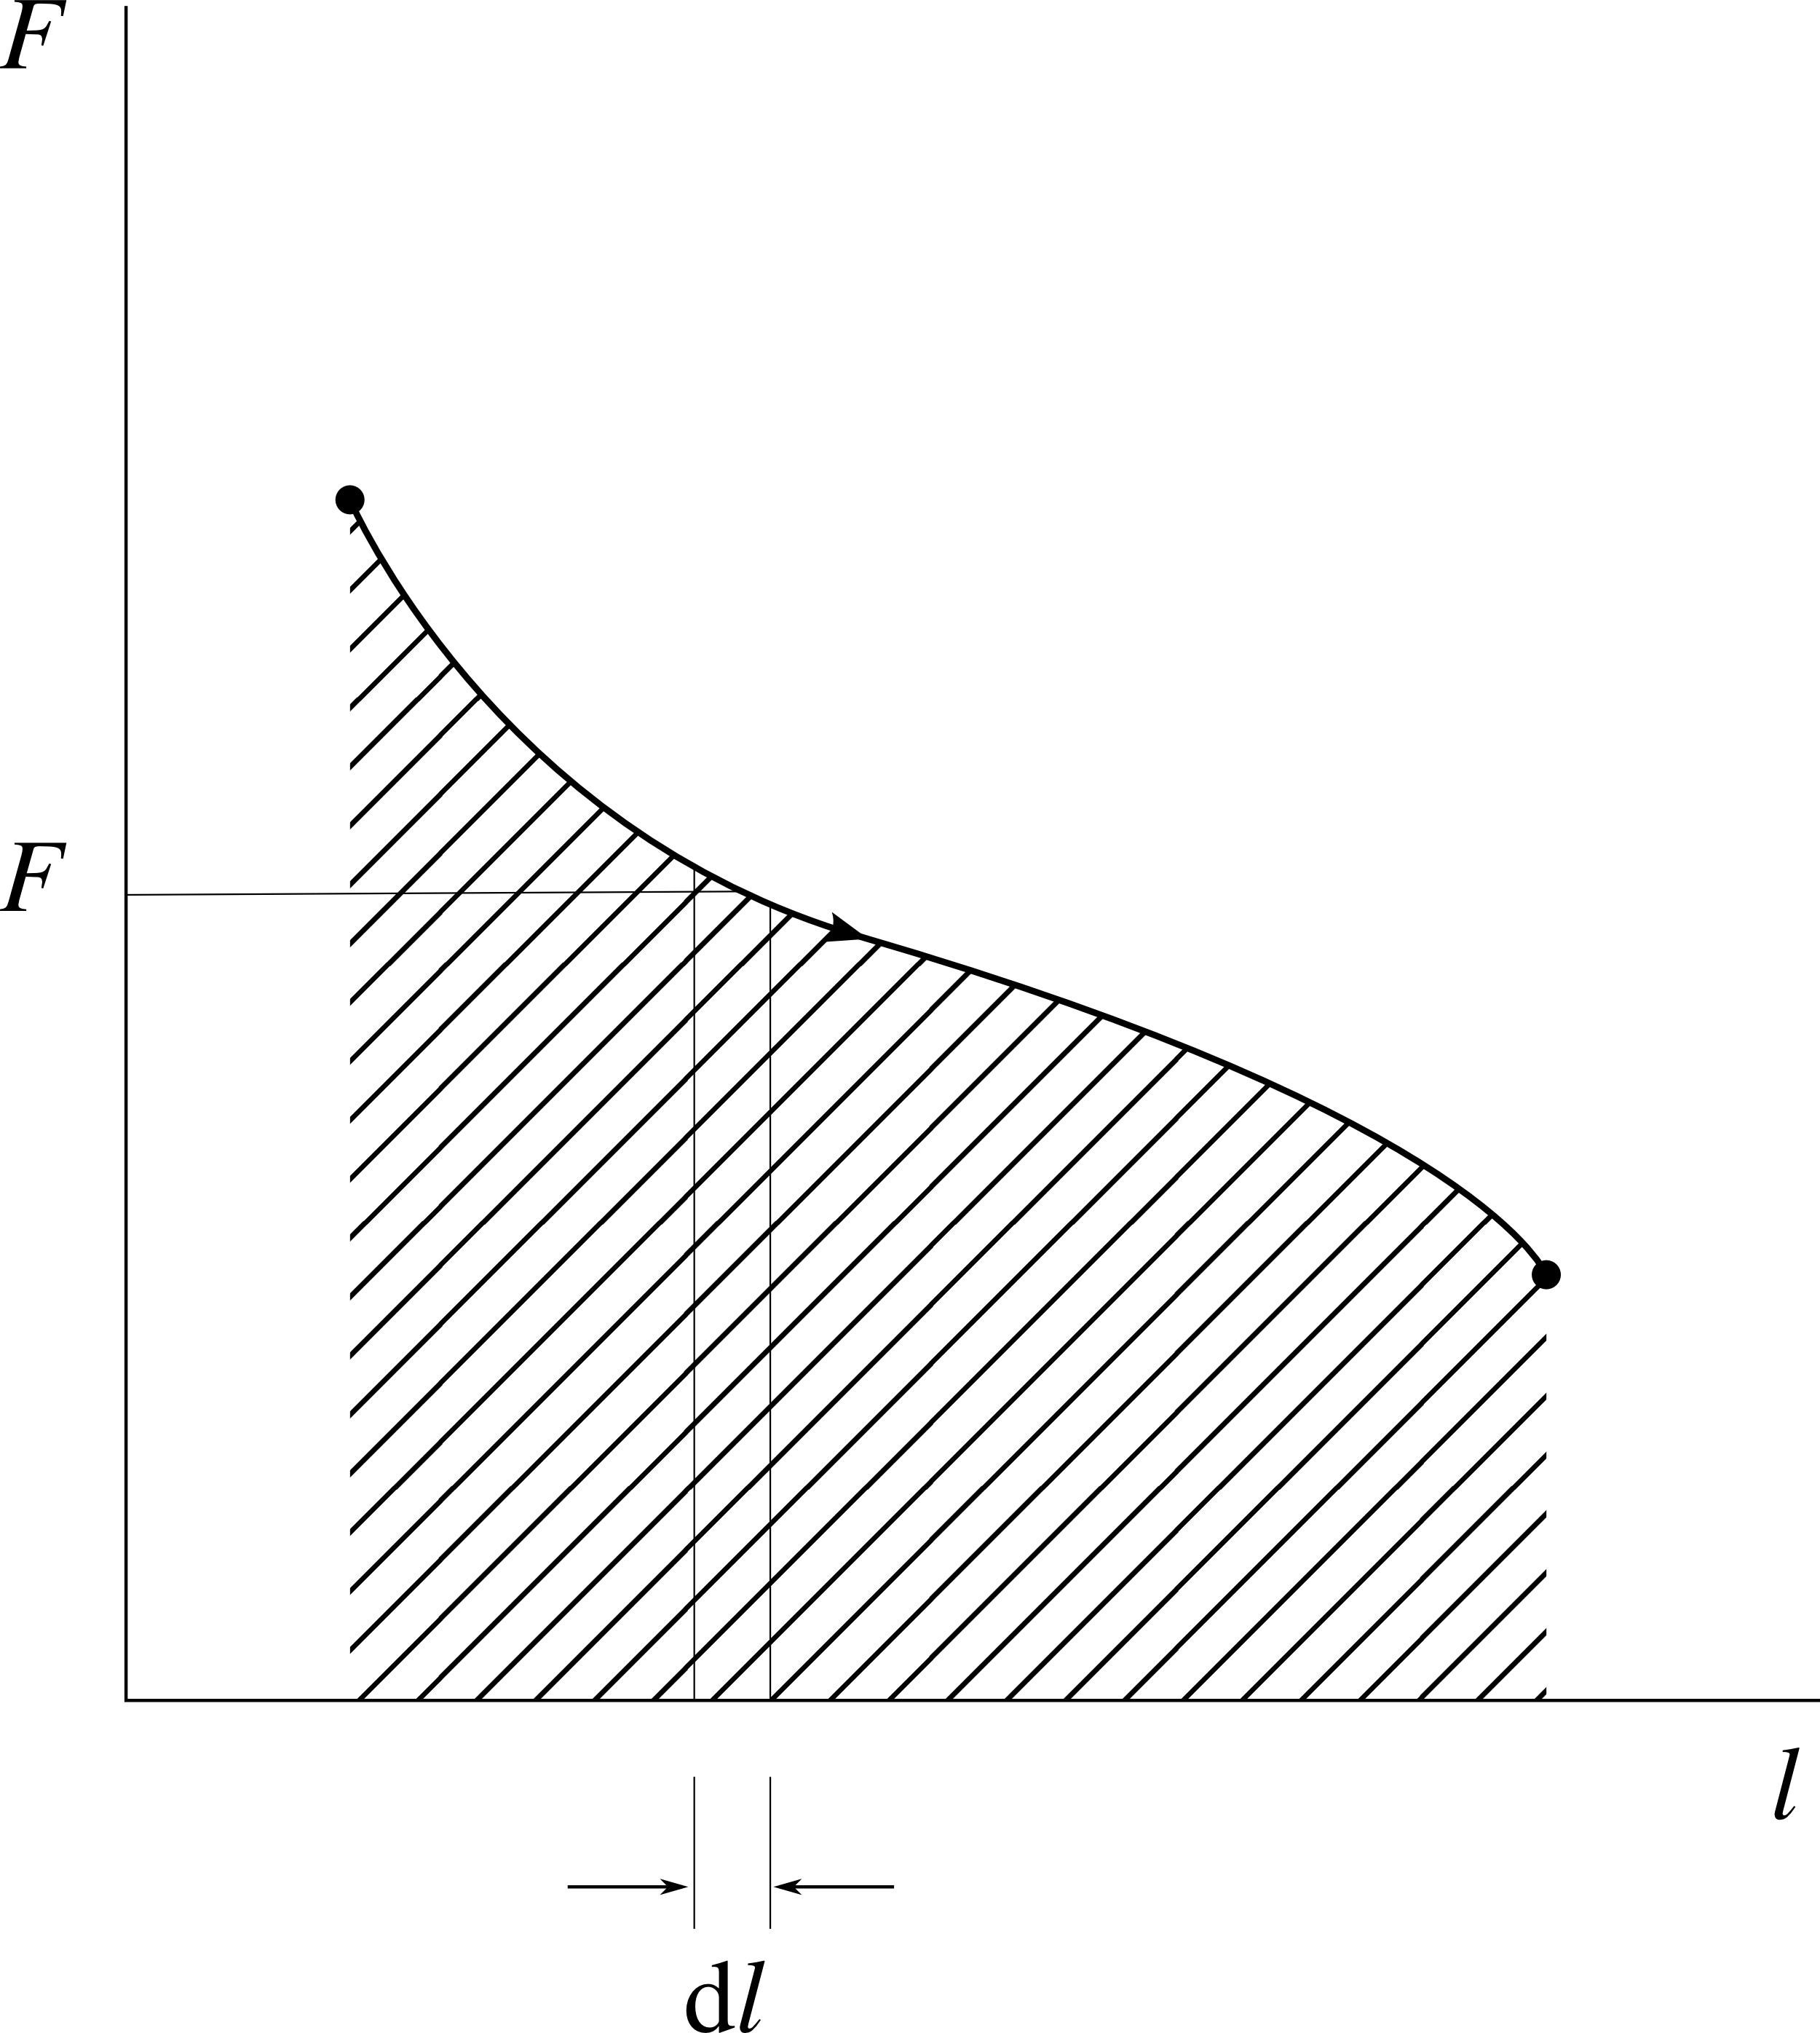
\includegraphics[width=10cm]{images/graph_force_deplacement.png}
	\end{center}
	\caption{Le travail fourni par un objet peut être visualisé avec l’aire sous la courbe force-déplacement. Dans le cas montré ici, l’objet voit sa longueur $l$ augmenter, et le travail sera négatif (fourni par l’objet).}
	\label{fig_force-déplacement-aire}
	\end{figure}

		\clearfloats
		\begin{anexample}
			Un ressort est comprimé depuis une longueur de \SI{30}{\centi\metre} jusqu’à une longueur de \SI{5}{\centi\metre}. Le ressort est tel qu’il exerce une force (en \si{newtons}) indépendante de sa longueur et égale à
				\begin{equation*}
					F_{(l)} = \SI{6e3}{\newton}
				\end{equation*}
			Quelle est l’énergie fournie au ressort sous forme de travail pendant la compression ?
				
				\begin{answer}
					Le transfert de travail s’obtient avec l’\cref{eq_travail_fdl}, en prenant soin de poser les bornes en unités \textsc{si} : 
					$ W_\fromatob = - \int_\A^\B F_{(l)} \diff l = - \int_\A^\B \num{6e3} \diff l = - \num{6e3} \int_\A^\B \diff l = - \num{6e3} \left[l\right]_{l_\A}^{l_\B } = -\num{6e3} (\num{0,05} - \num{0,3}) = \SI{+1,5e3}{\joule} = \SI{+1,5}{\kilo\joule}.$
						\begin{remark} Le signe du travail transféré est positif : le ressort a \emph{reçu} de l’énergie. Cela ne nous surprend pas : sa longueur a diminué, pendant qu’il se faisait comprimer.\end{remark}
						\begin{remark} Les ressorts possédant une telle caractéristique (indépendante de leur longueur) sont souvent des ressorts en ruban, comme ceux alimentant les montres mécaniques. \end{remark}
				\end{answer}
		\end{anexample}

		\begin{anexample}
			Un autre ressort est comprimé depuis une longueur de \SI{30}{\centi\metre} jusqu’à une longueur de \SI{5}{\centi\metre}. Il est tel qu’il exerce une force (en \si{\newton}) liée à sa longueur $l$ (en~\si{\metre}) par la relation :
				\begin{equation*}
					F_{(l)} = \num{9e3} - \num{14e3} \ l
				\end{equation*}
			Quelle est l’énergie fournie au ressort sous forme de travail pendant la compression ?
				
				\begin{answer}
					Le travail effectué s’obtient toujours avec l’\cref{eq_travail_fdl}, dont l’intégrale est à peine plus complexe :
					$ W_\fromatob = - \int_\A^\B (\num{9e3} - \num{14e3} l) \diff l = - \left[\num{9e3} \ l - \frac{1}{2} \num{14e3} \ l^2\right]_{l_\A}^{l_\B } = -\num{e3} \left[9 l - 7 l^2\right]_{\num{0,3}}^{\num{0,05}} =  -\num{e3} (\num{0,4325} - \num{2,07}) = \SI{+1,6375e3}{\joule} = \SI{+1,638}{\kilo\joule}.$
						\begin{remark} Les ressorts possédant une telle caractéristique (force proportionnelle à la distance) sont souvent à spires régulières. \end{remark}
				\end{answer}
		\end{anexample}

		\begin{anexample}
			Un autre ressort est comprimé depuis une longueur de \SI{30}{\centi\metre} jusqu’à une longueur de \SI{5}{\centi\metre}. Il est tel qu’il exerce une force (en \si{\newton}) liée à sa longueur $l$ (en~\si{\metre}) par la relation :
				\begin{equation*}
					F_{(l)} = \num{14e3} - \num{12e3} \ l^{\num{0,3}}
				\end{equation*}
			Quelle est l’énergie fournie au ressort sous forme de travail pendant la compression ?
				
				\begin{answer}
					Le travail effectué s’obtient encore et toujours toujours avec l’\cref{eq_travail_fdl},\\ 
					$ W_\fromatob = - \int_\A^\B (\num{14e3} - \num{12e3} \ l^{\num{0,3}} ) \diff l = - \num{e3} \left[\num{14} \ l - \frac{1}{\num{0,3}+1} 12 \ l^{\num{0,3}+1} \right]_{\num{0,3}}^{\num{0,05}} = -\num{e3} \ (\num{0,5121} - \num{2,2703}) = \SI{+1,7582e3}{\joule} = \SI{+1,758}{\kilo\joule}.$
						\begin{remark} Les ressorts possédant une telle caractéristique sont à spires progressives : très souples au départ, mais augmentant rapidement en dureté. Ils sont souvent utilisés dans les suspensions d’automobiles. Nous verrons au \coursdeux que les gaz on une caractéristique similaire.\end{remark}
				\end{answer}
		\end{anexample}



\section{La chaleur}

	\subsection{La température}
	\label{ch_définition_température_cours1}

		Nous définissons temporairement la \vocab{température} comme étant le potentiel d’un corps à fournir ou recevoir de la chaleur.

		La température d’un corps est une grandeur qui indique son niveau d’excitation interne. Plus ses molécules possèdent d’énergie cinétique, avec des vitesses de direction différente, et plus sa température sera grande. 

		Lorsque les molécules constituant un corps sont parfaitement immobiles les unes par rapport aux autres, le corps n’a plus de vibration interne : cet état définit la température zéro. À l’inverse, l’échelle de température est ouverte vers l’infini. On ne définit pas de point de température maximale.

		On ne peut pas mesurer simplement «~l’énergie cinétique moyenne des molécules~» d’un corps et il suit qu’il est très difficile de définir rigoureusement une échelle de température (par exemple, ce que représente une température «~deux fois plus grande~»). Nous reviendrons sur la notion même de température au \coursquatre et nous la définirons tout à fait au \courssept. Nous admettrons, dans cette attente, la définition plus haut.

		La température se mesure en \si{kelvins} (\si{\kelvin}), sur une échelle créée pour les besoins de la thermodynamique et fort peu modestement qualifiée d’\vocab{absolue}.

		L’étudiant/e aura probablement l’habitude d’utiliser une échelle en \si{degrés} \si{Celsius}~(\si{\degreeCelsius}). Elle précède l’échelle absolue en \si{kelvins}, mais a été habilement redéfinie et synchronisée avec cette dernière en 1848%
			\footnote{Nous aurons l’occasion d’étudier ce magnifique tour de passe-passe au \courssept.}%
		. Il suffit de soustraire 273,15 unités à une température absolue (en \si{kelvins}) pour lire une température en \si{degrés} \si{Celsius} :
		\begin{equation}
			T(\si{\degreeCelsius})\ \equiv \ T(\si{\kelvin}) - 273,15
			\label{def_température_kelvins_celsius}
		\end{equation}

		Les puristes remarqueront que l’unité est nommée \si{kelvin} et non «~degré Kelvin~». Quelques températures indicatives sont recensées dans le \cref{tab_temperatures}.

		\begin{table}
		\centering
		\renewcommand{\tabcolsep}{0.8em}
		\renewcommand{\arraystretch}{1.3}
		\sisetup{table-number-alignment=center-decimal-marker} %in this table, we don’t care about alignment
		\begin{footnotesize}
		\begin{spacing}{1}
		\begin{innersidebox}
		\begin{tabularx}{15.5cm}{@{}S@{}S|p{8.5cm}@{}} % the @{something} kills the inter-column space and replaces it with "something"
% last column width has to be set manually ; will break if margins change.
% L column in tabulary solves this but tabulary precludes using arydshln
			\toprule
			{\si{kelvins}} & {\si{degrés} \si{Celsius}} & ~ 	\\ % accolades allow escaping from the S column number alignment rules
			\midrule
			0		& -273,15	&	Zéro absolu (par définition) \\
			10e-11	& -273.1499999999	& Température la plus basse jamais atteinte (quelques particules seulement) \\
			4,22	& -268,93	& Ébullition de l’hélium à pression atmosphérique \\
			44	& -229		& Température moyenne de la surface de Pluton* \\
			184	& -89,4		& Température atmosphérique minimale enregistrée sur Terre* \\
			273,15	& 0		& Fonte de l’eau à pression atmosphérique \\
			327	& 54		& Température atmosphérique maximale enregistrée sur Terre* \\
			373,15	& 100		& Ébullition de l’eau à pression atmosphérique \\
			400	& 127		& Température du nez d’un Concorde en croisière* \\
			483	& 200		& Four domestique ordinaire* \\
			485	& 210		& Auto-inflammation du carburant diesel* \\
			753	& 480		& Température des bords d’attaque d’un SR-71 en croisière* \\
			1100	& 830		& Feu de bois* \\
			1900	& 1600		& Température du bouclier d’une navette spatiale en ré-entrée atmosphérique* \\
			2500	& ~		& Filament d’une lampe à incandescence \\
			5000	& ~		& Fonte du diamant (à~\SI{12}{\giga\pascal}) \\
			5800	& ~		& Surface du soleil \\
			16e6	& ~		& Centre du soleil \\
			350e6	& ~		& Au sein de la déflagration d’une arme nucléaire \\
			3e9	& ~		& Cœur d’une grosse étoile à son dernier jour \\
			1e12	& ~		& Particules en collision au sein du RHIC \\
			1.417e32	& ~	& L’univers \SI{5,391e-44}{\second} après le Big Bang \\
			\hline 
		\end{tabularx}
		\end{innersidebox}
		\end{spacing}
		\end{footnotesize}
		\caption{Quelques exemples de températures. Les astérisques dénotent une conversion approximative (liée à la précision des valeurs).}
		\sisetup{table-number-alignment=center} % back to setting specified in our stylesheet
		\label{tab_temperatures}
		\end{table}
		
		
	\subsection{La chaleur}
	
		\thermoquotebegin{O}
			Ces résultats sont inexplicables si nous considérons que la chaleur est une substance.\nolinebreak\makebox(18,5){\color{gray}\scalebox{2}{»}}\par\vspace{-0.3cm}\begin{flushright}James Joule, 1845\\\textit{On the Changes of Temperature Produced by the Rarefaction and Condensation of Air}~\cite{joule1845}\end{flushright}\vspace{-1em}
		%\thermoquoteend{James Joule, 1845}{\textit{On the Changes of Temperature Produced by the Rarefaction and Condensation of Air}~\cite{joule1845}}
		%\thermoquotebegin{O}
		\makebox(18,5){\color{gray}\scalebox{2}{«}}
			Ces circonstances […] nécessitent une comparaison entre travail et chaleur, qu’il nous faut effectuer en partant de l’hypothèse divergente que la production de travail est due non seulement à un changement dans la \emph{distribution} de la chaleur, mais aussi à une \emph{consommation} de celle-ci ; et inversément, que par la consommation de travail la chaleur puisse être \emph{produite}.
		\thermoquoteend{Rudolf Clausius, 1850}{\textit{Über die bewegende Kraft der Wärme und die Gesetze, welche sigh daraus für die Wärmelehre selbst ableiten lassen} \mbox{\cite{clausius1850, clausius1850en, clausius1850fr}}}

		Lorsque l’on met deux corps de températures différentes en contact, leurs températures ont tendance à s’égaliser au cours d’un transfert spontané d’énergie. Nous appelons cette forme d’énergie la \vocab{chaleur}.

		La chaleur, notée $Q$, est \textbf{une forme d’énergie} (mesurée en \si{joules}). À l’échelle macroscopique, c’est un transfert d’énergie sous forme chaotique. On peut le provoquer de plusieurs façons, dont les plus pertinentes pour l’ingénieur/e sont :

		\begin{itemize}
		
			\item la perte d’énergie interne d’un corps, par mise en contact avec un corps de température plus basse ;

			\item le frottement ;
			
			\item la disparition de masse au sein d’une réaction nucléaire ;
			
			\item la transformation d’énergie potentielle entre atomes, par réaction chimique (en particulier la combustion d’hydrocarbures avec l’oxygène atmosphérique). 

		\end{itemize}
		
		De même que l’on note $Q$ la chaleur (\si{\joule}), on note $q$ la \vocab{chaleur spécifique} (\si{\joule\per\kilogram}).
		
		La notion de chaleur est très difficile à appréhender. On l’a longtemps crue être un fluide (le \textit{calorique}) de densité très faible, capable d’imprégner tous les matériaux. Cette théorie a été abandonnée au milieu du \textsc{xix}\ieme siècle, lorsque l’on a mis en évidence que \textit{la chaleur n’est pas conservée}, c’est-à-dire qu’elle a une capacité à disparaître ou apparaître. Par exemple, un moteur en marche reçoit de la chaleur (par combustion) mais il en rejette moins qu’il n’en a reçu. Il en transforme une partie en travail, que l’on utilise par exemple pour propulser un véhicule. \\
		À l’échelle microscopique (lorsque l’on considère le mouvement individuel des particules) les concepts de température et de chaleur sont encore plus difficiles encore à définir ; mais cela dépasse le domaine d’étude de cet ouvrage\footnote{Pour mieux définir les frontières entre les échelles macroscopique et microscopique dans la thermodynamique de l’ingénieur, les étudiants les plus rigoureux pourront par exemple consulter l’ouvrage d’Alexandre Watzky~\cite{watzky2007}. Richard Feynman~\cite{feynman1963, feynman1963fr} explore à plusieurs reprises ces changements d’échelle et leurs implications.}\nolinebreak.


	\subsection{La capacité thermique}
	\label{ch_capacite_thermique}

		Lorsque l’on fournit la même quantité de chaleur à deux corps différents, leur température peut augmenter de différente façon -- par exemple, il faut moins de chaleur pour augmenter de~\SI{1}{\degreeCelsius} la température d’un \si{kilogramme} d’acier que d’un \si{kilogramme} d’aluminium. Cette propension de la température à augmenter est nommée \vocab{capacité thermique} (ou \vocab{capacité calorifique}).

		On définit la capacité thermique massique d’un corps comme la quantité de chaleur nécessaire pour augmenter d’un \si{kelvin} la température d’un \si{kilogramme} de ce corps :
		\begin{equation}
			c\ \equiv \ \frac{\diff q}{\diff T} = \frac{1}{m} \frac{\diff Q}{\diff T}
			\label{eq_def_capacité_calorifique_massique}
		\end{equation}

		\begin{equationterms}
			\item où \tab ~~$c$ \tab\tab est la \vocab{capacité thermique massique} du corps considéré (\si{\joule\per\kilogram\per\kelvin}),
			\item \tab $\diff q$ \tab est une quantité spécifique infinitésimale de chaleur (\si{\joule\per\kilogram}),
			\item et \tab $\diff T$ \tab est une variation infinitésimale de température (\si{\kelvin} ou \si{\degreeCelsius}).
		\end{equationterms}

		La capacité calorifique massique des solides est en général invariante. Par contre, pour les fluides, que nous utilisons beaucoup dans les machines, ce n’est pas si simple :

		\begin{itemize}

			\item En faisant travailler un gaz (c’est-à-dire en le laissant pousser sur une paroi mobile), on augmente nettement sa capacité calorifique massique. Nous quantifierons ces propriétés au \coursquatre ;

			\item La capacité calorifique massique des liquides et vapeurs devient infinie~(!) pendant l’ébullition, qui a lieu sur une plage particulière de propriétés. Hors de cette plage, la capacité redevient finie mais elle varie avec la température. Nous décrirons ces comportements au \courscinq.

		\end{itemize}

		\begin{anexample}
			La capacité calorifique massique de l’acier solide est constante (indépendante de la température) et a pour valeur $c_{\text{acier}} = \SI{475}{\joule\per\kilogram\per\kelvin}$. 
			
			Combien faut-il de chaleur pour faire passer un bloc de \SI{50}{\kilogram} d’acier depuis une température $T_\A = \SI{5}{\degreeCelsius}$ jusqu’à une température $T_\B = \SI{18}{\degreeCelsius}$ ?
				\begin{answer}
					Nous utilisons la définition \ref{eq_def_capacité_calorifique_massique} pour écrire, dans le cas général :
						\begin{IEEEeqnarray*}{rCl}
							c_{\text{acier}} 				&=& \frac{1}{m_{\text{acier}}} \frac{\diff Q}{\diff T}\\
							\diff Q 							&=& c_{\text{acier}} \ m_{\text{acier}} \diff T\\
							Q_\fromatob						&=& \int_\A^\B m_{\text{acier}} \ c_{\text{acier}} \diff T
						\end{IEEEeqnarray*}
					Comme la capacité $c_{\text{acier}}$ est indépendante de $T$ cette intégrale devient simplement :
					$ Q_\fromatob = m_{\text{acier}} \ c_{\text{acier}} \int_\A^\B \diff T = m_{\text{acier}} \ c_{\text{acier}} (T_\B - T_\A ) = 50 \times 475 \times (18 - 5) = \SI{+3,0875e5}{\joule} = \SI{+308,8}{\kilo\joule}$.
						\begin{remark}Pendant l’intégration, $\int_\A^\B \diff T$ devient $\Delta T$ (une différence de température), tandis que $\int_\A^\B \diff Q$ devient seulement $Q_\fromatob$ (un transfert entre deux états). La chaleur n’est pas «~diminuée~», elle est transmise. Nous prenons l’habitude d’expliciter le signe des transferts.\end{remark}
						\begin{remark}Une conversion des deux températures en \si{kelvins} n’aurait pas changé la valeur du $\Delta T$. Le résultat serait bien sûr identique.\end{remark}
						\begin{remark}Avec une résistance électrique de la puissance d’un radiateur domestique ordinaire (\SI{2}{\kilo\watt}), il faudrait $\Delta t = \frac{Q_\fromatob}{\dot Q} = \frac{\num{308,8e3}}{\num{2e3}} = \SI{154}{\second}$ pour réchauffer l’acier, soit un peu plus de deux minutes. Nous verrons au \coursquatre que l’air à pression constante a une capacité calorifique massique trois fois plus grande que celle de l’acier.\end{remark}
				\end{answer}
		\end{anexample}


\section{Le chaud et le froid}

	Nous terminons ce chapitre en re-visitant quelques termes de langage courant tels que nous les comprenons en thermodynamique :

		\begin{description}

			\item \textit{Le chaud} --- Pour nous, «~chaud~» n’est pas une propriété des corps : plutôt que «~cet objet est chaud~» nous dirons qu’il est à haute température. Plutôt que «~cet objet s’échauffe/se refroidit~» nous dirons que sa température augmente ou diminue.\\
				Dans le langage courant, les expressions comme «~il fait chaud~» ou «~les grandes chaleurs~» font également allusion à la température.
			
			\item \textit{Chauffer} --- Pour nous, «~chauffer~» c’est fournir de la chaleur. On peut «~chauffer~» un corps pendant que sa température chute. On peut également faire augmenter la température d’un corps sans lui apporter de chaleur (\cref{fig_chauffer_refroidir}).

		\begin{figure}
			\begin{center}
			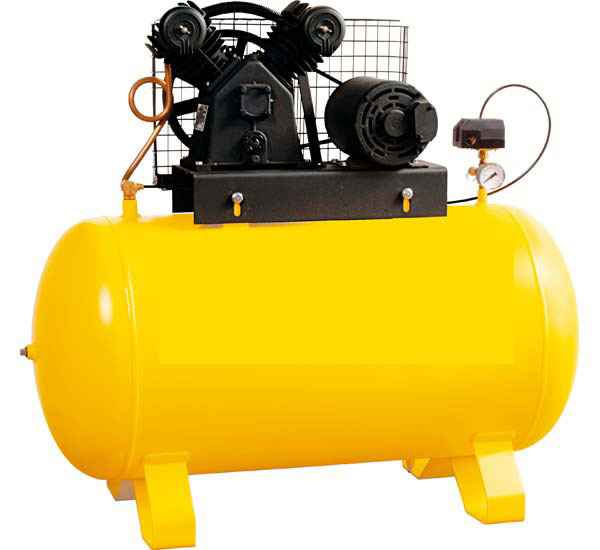
\includegraphics[height=0.38\textwidth]{images/air_piston_compressor.jpg}
			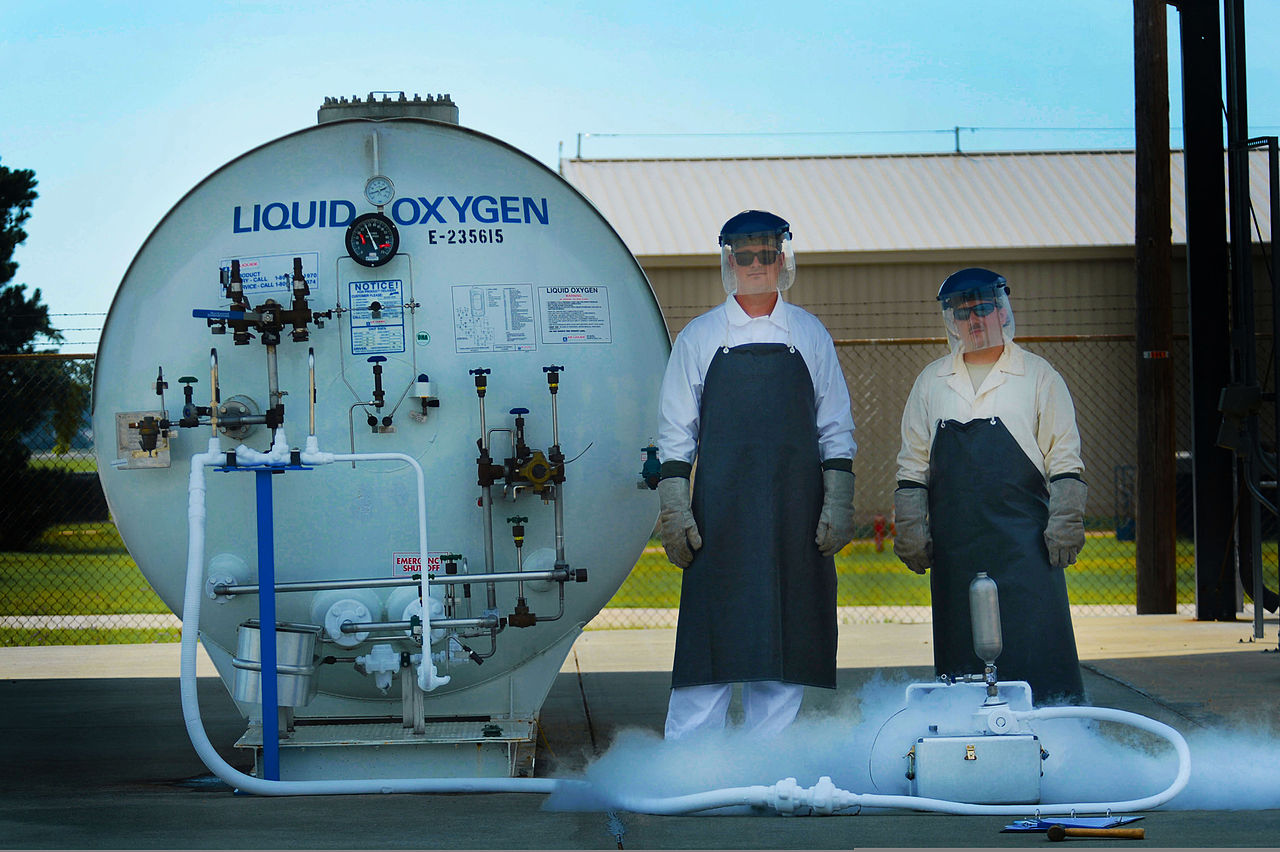
\includegraphics[height=0.38\textwidth]{images/liquid_oxygen_expansion.jpg}
			\end{center}
			\supercaption{Lorsqu’il est comprimé dans un compresseur, l’air perd de la chaleur au travers des parois et des aubes des cylindres ; et pourtant sa température augmente.\\
			À l’inverse, lorsqu’il est détendu dans une soupape, l’oxygène liquide reçoit de la chaleur de l’atmosphère (comme le mettent en évidence la condensation et le gel de l’eau atmosphérique sur les tuyaux) ; et pourtant sa température chute.}{\wcfile{Compressor3.jpg}{Photo compresseur} \ccbysa Fábio Teixeira\\ \wcfile{U.S. Air Force Tech. Sgt. Jason Powers, left, a noncommissioned officer in charge with the 20th Logistics Readiness Squadron (LRS), and Staff Sgt. Adam Rozell, a fixed facilities supervisor with the 20th LRS 140626-F-SX095-017.jpg}{Photo oxygène liquide} \pd Jensen Stidham / USAF}
			\label{fig_chauffer_refroidir}
		\end{figure}
			
			\item \textit{Le froid} --- Pour nous, la sensation de «~froid~» indique une faible température. Nous ne considérerons pas «~le froid~» comme étant quelque chose que l’on peut fabriquer ni mesurer. Nous dirons plutôt que nous prélevons de la chaleur d’un corps (par exemple, un réfrigérateur prend de la chaleur à  d’un aliment tiède). 
			
			\item \textit{Le feu} --- Le feu est le nom donné au dégagement de lumière (rayonnement électromagnétique) par un gaz à haute température. En thermodynamique, le «~feu~» n’a aucune propriété particulière. Il s’agit pour nous de la même chaleur qu’elle soit dégagée par combustion de bois, de kérosène, par frottement dans un frein, ou par une réaction nucléaire. Seule compte au final la température à laquelle elle est transmise !
			\end{description}

				\thermoquotebegin{o}
					Le principe à suivre pour construire une échelle de température peut tout d’abord paraître évident, puisqu’il peut apparaître qu’un thermomètre parfait ferait correspondre des ajouts de chaleur égaux à des élévations égales de température, mesurées par les graduations de son échelle. Il est toutefois désormais reconnu comme fait établi par l’expérience (par la variation des capacités calorifiques des corps) que la thermométrie sous ce précepte est impossible, et nous n’avons plus de principe sur lequel fonder une échelle thermométrique absolue.
				\thermoquoteend{William Thomson\\{\tiny(non encore couronné \textit{Baron Kelvin}…)}}{1848~\cite{kelvin1848}}
				\vspace{-0.7em}~\vspace{-1.8em}%FIXME -- hack pour faire tenir la citation sur le côté
			\begin{description}
			\item \textit{Le thermomètre} --- Nous laissons à l’étudiant/e le loisir d’explorer le fonctionnement des \vocab{thermomètres} : comment peut-on \emph{savoir} dans l’absolu qu’une température est haute ou basse ?\\
				Nous nous contentons de remarquer que nous sommes nous-mêmes de très mauvais thermomètres : comme le corps humain s’efforce de se maintenir à température constante, nos sensations de «~chaud~» ou de «~froid~» sont intrinsèquement liées aux transferts de chaleur.

		\end{description}
		
	Même si ce vocabulaire nous place probablement au rang des scientifiques insociables relégués aux bouts de table, il nous équipe mieux pour affronter la suite, car au chapitre prochain, nous attaquons les \textit{systèmes fermés}.

